\documentclass[a4paper]{article}
\usepackage[utf8]{inputenc}
\usepackage{pdfpages}
\usepackage{arxiv}

\usepackage[utf8]{inputenc} % allow utf-8 input
\usepackage[T1]{fontenc}    % use 8-bit T1 fonts
\usepackage{hyperref}       % hyperlinks
\usepackage{url}            % simple URL typesetting
\usepackage{booktabs}       % professional-quality tables
\usepackage{amsfonts}       % blackboard math symbols
\usepackage{nicefrac}       % compact symbols for 1/2, etc.
\usepackage{microtype}      % microtypography
\usepackage{lipsum}
\usepackage{marvosym}
\usepackage{makecell}
\usepackage{xcolor}
\usepackage{graphicx}
\usepackage{epsfig}
\usepackage{fontawesome}
\usepackage[stable]{footmisc}
\usepackage{amssymb}
\usepackage[affil-it]{authblk}

\renewcommand\theadalign{bc}
\renewcommand\theadfont{\bfseries}
\renewcommand\theadgape{\Gape[4pt]}
\renewcommand\cellgape{\Gape[4pt]}
\begin{document}


\title{Formal Machines for Length Prefix Languages\\{\small Calc-PDAs for Netstrings and Google's Protocol Buffers}}
\author{Jannis Leuther}
\affil{Bauhaus-Universität Weimar}
\date{09/2019}

\maketitle

% Abstract
\begin{abstract}
    This bachelor's thesis presents the results of research about language based security in the field of data serialization. Particularly, length-prefix formats are analyzed, which are a prominent form of serializing distinguishable messages in a data stream. These formats prepend a numerical value before the actual message representing the length of the message. Due to the lack of a theoretical, fundamental language class for length-prefix formats, many bugs, errors and also severe security vulnerabilities in existing implementations have appeared and sometimes been exploited in the past. By establishing a new language class called Calc-LL(1), we are trying to improve security and eliminate errors in length-prefix serialization. We approached this subject matter by using an existing definition for a less complex length-prefix language class, Calc-regular languages, as the starting point for our research. \\\\
    The main contribution reviewed in this thesis is the creation of a formal machine for the new length-prefix language class Calc-LL(1) in form of an extended definition of a pushdown automaton, the Calc-PDA. By augmenting a regular pushdown automaton with additional features such as conditions and operations, a Calc-PDA is able to detect malformed length-prefix messages in a serialized data stream. There are plenty possibilities of such a message being malformed, the most prominent example as seen with the 'Heartbleed' bug in 2014, is some message content where its size does not match the length prefix. The Calc-PDA was implemented exemplarily for two formats which are used in practice in the real world: Netstrings and Google's Protocol Buffers. Additionally, besides the definition of a Calc-PDA, we started to construct an equivalent grammar definition for Calc-LL(1) languages, a Calc-EBNF. So far, it was created for both of our exemplary formats, but a universal definition is desired eventually, just as with Calc-PDAs.\\\\
    We hope that these findings can add more to the superior goal of constructing a fundamental approach to length-prefix serialization handling. Ultimately, this can help eliminate countless bugs and help guarantee security for machines and users worldwide.
\end{abstract}

% Table of contents, List of figures, List of tables
\newpage
\tableofcontents
\listoffigures
\listoftables

% First page
\newpage
\section{Introduction}
\label{1.0}
\subsection{Roadmap}
\label{1.1}
We will begin by covering the foundations of this research topic by explaining some fundamental prerequisites as well as going over the motivation that led to this research. After this, we will be introducing two exemplary formats which tie our mostly theoretically based research to the real world. Chapter two revisits Calc-regular languages explaining them briefly. These findings by Grosch, Koenig, Lucks \cite{Calc-regular-paper} represent a starting point for our own research, as we will be benefiting greatly from these already established results related to our topic. In the following chapter, a new language class 'Calc-LL(1)' is introduced by us and defined informally by also revisiting LL(1) parsing techniques and referring to some basic work done in an earlier project by the author of this thesis. The most significant results of the research highlighted in this thesis get presented in chapter four by showcasing the concept of an automaton for Calc-LL(1) languages, a 'Calc-PDA'. The structure of such an automaton is explained and two example machines are shown that are based on the two representative formats that were already introduced in chapter one: netstrings and Google's protocol buffers. Following this is a clear breakdown of the formal definition of Calc-PDAs. In the subsequent chapter, a proposition for Calc-LL(1) grammars is made, establishing 'Calc-EBNFs' based on the extended Backus-Naur form for our example formats.
Finally, a summarization will be given as well as the important lookout to future projects that can build upon this thesis' results and findings.\\\\
To fully grasp the research presented in this thesis, some basic knowledge about concepts from formal language theory, automatons and their usage in parsing as well as data serialization is recommended. Fundamental skills in formal language theory and formal automatons for regular and context-free languages\footnote{As per Chomsky hierarchy \cite{Chomsky-Hierarchy}.} are presupposed and not covered. In the first chapter, though, we will be establishing the core foundations of this thesis by also briefly explaining what data serialization means and how our research affects certain areas of this procedure.

\subsection{Length-Prefix Notation in Binary Data Serialization}
\label{1.2}
Computers that communicate with each other can only do so by using the binary system. Let's suppose some party $A$ wants to send a package of messages encoded in UTF-8 to $B$. First of all, $A$ has to convert these messages to its binary representation (serialization), then they can distribute these messages to $B$, who deserializes them to get their original form.
The very basic concept on which the motivation for this thesis is based on revolves around data serialization. Particularly, we will be looking at binary data and its structural representation after being serialized, or vice versa, prior to being deserialized.
Since binary data evidently only relies on two characters, \texttt{0} and \texttt{1}, there exist no symbols that can act as delimiters or punctuation marks in any binary data stream. This fact makes it very challenging for any receiver of data including multiple messages to determine where each of these messages end and/or another one starts. In order to deal with this issue, several binary notations have been established. We will be looking at one of these formats called 'length-prefix notation'. \\\\
Length-prefix notation solves the aforementioned problem by inserting a length field at the beginning of each message, before the actual content. This length field guarantees that any machine which parses a binary data stream for deserialization can identify the length of a current message in the data stream. This also means that given the length of the upcoming serialized message, the parser can calculate at which byte in a data stream this message ends and therefore also where the next one begins. This concept is employed in various known and lesser known data formats, such as 'Google protocol buffers' \cite{google-protobuf-overview}, 'Abstract Syntax Notation One (ASN.1)' \cite{ASN.1}, Portable Network Graphics (PNG) \cite{PNG}, the binary representation of JSON, 'BSON'\cite{BSON-overview}, 'netstrings' \cite{netstrings} and many others.

\subsection{Vulnerabilities in Length-Prefix Languages}
\label{1.3}
Incorrect parsing of length-prefix languages can lead to severe security faults, as seen with the famous 'Heartbleed' exploit. 
This serious bug in the \textit{OpenSSL} cryptographic software library surfaced in 2014 \cite{heartbleed-wiki}. The security vulnerability was the result of a flawed implementation of the so called 'heartbeat' functionality in the library which was added 2 years earlier, in 2012.\\ 
To test if another party $Y$ was still alive, a party $X$ sends a 'heartbeat' package to $Y$ using the binary interface ASN.1 \cite{ASN.1}. This package's structure includes a length-prefix $\ell$ which corresponds to the size of the payload $M_x$. To signal that they are still alive, $Y$ then responds with a similarly formed package including $\ell$ and $M_y=M_x$. Crucially, $Y$ must detect and ignore incorrectly formed packages, $e.g.$, when the size of $M_x$ is bigger than $\ell$ indicated.
\\\\However, $Y$ failed to verify if the length $\ell$ of the length-prefix actually corresponds to the size of the payload $M_x$.
An attacker could therefore send short 'heartbeat' packages to $Y$ with $\ell$ being a significantly larger number than the size of $M_x$. $Y$ does not detect this malformed package and responds with the package expecting the message to be of size $\ell$. As $|M_x| << \ell$, party $Y$ now fills the rest of the message $M_y$ with bytes from the internal storage until $|M_y| = \ell$ is reached. This compromises $\ell-|M_y|$ bytes of $Y$'s internal memory \cite{Heartbeat-info}\cite{heartbleed-site}. \\\\
Heartbleed is the most prominent example on why a fundamental and formally correct definition for length-prefix languages is necessary. Using these foundations, many errors and security concerns can be avoided, especially also when considering cross-format communication.

\subsection{Netstrings}
\label{1.4}
To efficiently work with length-prefix languages and grasp their challenges, many formats lend themselves to be used as working examples. Throughout this thesis, two formats will appear repeatedly, 'netstrings' and 'Google protocol buffers' \cite{google-protobuf-overview}.\\\\
Netstrings \cite{netstrings} represent a simple encoding of self-delimiting strings using length-prefix notation. Every netstring message is built sequentially as follows:
\begin{itemize}
    \item a length-prefix $\ell$ in decimal representation,
    \item a colon (":"), separating the length-prefix from the content,
    \item the content, an arbitrary string consisting of $\ell$ bytes,
    \item a comma (","), marking the end of the netstring structure.
\end{itemize}
The string \texttt{"Hello World"}, including the space between the two words, gets encoded to "\texttt{11:Hello World,}", including the comma after "\texttt{World}". Netstrings allow recursive usage, also called nesting. This means that one netstring can act as a container for another netstring. $E.g.$, both strings "\texttt{Hello}" and "\texttt{World}" included in a netstring acting as a container get encoded to "\texttt{16:5:Hello,5:World,,}". Keep in mind that the double comma after "\texttt{World}" is necessary, as one comma acts as the end-of-content symbol for the inner netstring and the last comma acts as the end-of-content symbol for the outer netstring which acts as the container. In this example, the nesting depth of 1 needed to be known beforehand. A nesting depth of 0 would signal that this structure represents one netstring of size 16 including the string "\texttt{5:Hello,5:world,}". Using the original specifications by D.J. Bernstein \cite{netstrings}, there exists no type-field in netstrings. Therefore, with these original specifications, the depth of nesting needs to be predetermined before parsing. A 'Heartbleed' package encoded as a netstring with payload $M=\texttt{"payload"}$ and padding \texttt{"padding"} would be "\texttt{17:7:payload,padding,}" with a nesting depth of 1. A malformed package used for the 'Heartbleed' attack could be "\texttt{6:9999:,,}".\\\\
Fixed nesting in netstrings is rather unpractical since the information about nesting depth has to be encoded and parsed separately before parsing the netstring itself. Therefore, we extended the definition for netstring slightly, so that variable nesting can be allowed. This means that the parser does not need to know any information about the nesting depth beforehand. As netstrings can act as either a simple netstring or as a container of other netstrings or containers, we can signal the parser at the start of every length-prefix which role this specific netstring will take. By prepending a zero (\texttt{0}) before the length-prefix, we mark this netstring as a container. We only allow the appearance of at most one leading zero in the length-prefix. A netstring with a nesting depth of 2 could look like "\texttt{012:08:5:Hello,,,}". The parser can parse this netstring without any prior knowledge of its nesting depth and still knows that this specific netstring represents a simple netstring of length 5 embedded in a container of size 8 which is then also embedded in another container of size 12.\\\\
While in Grosch et al.'s paper about Calc-Regular languages \cite{Calc-regular-paper} a solution to the handling of length-prefix languages with fixed nesting was proposed, this thesis will be focused on the challenges of a secure definition of length-prefix languages employing variable nesting.
\subsection{Google Protocol Buffers (Protobufs)}
\label{1.5}
Google protocol buffers are a language and platform neutral data serialization format for use in communication protocols or data storage amongst other things \cite{google-protobuf-overview}. Protobufs are a prime example for a variably nested length-prefix language widely used in practice. Contrary to netstrings, protobuf is a schema-language and additionally includes a type-field which conveys information also related to the current schema it is based on \cite{google-protobuf-encoding}. This language also does not use any delimiters or end-of-content symbols and encodes type field, length field and content field in immediate sequence.\\\\
To give a brief example, the strings "Hello" and "World" in two sequential protobufs are encoded in hexadecimal ASCII representation to "\texttt{12 05 48 65 6C 6C 6F 0A 05 57 6F 72 6C 64}". The first byte (\texttt{12}) and the eighth byte (\texttt{0A}) represent the type-fields of the corresponding string encodings. Second (\texttt{05}) and ninth (\texttt{05}) byte represent the length-fields containing the length of the upcoming string, which are the next five bytes respectively. It is important to mention one of the major differences to netstrings: encoded in a stream with several messages followed by another, the type-field byte of the upcoming message comes immediately after the last byte of the content-field from the prior message encoding. Netstrings (and many other length-prefix languages), on the other hand, employ an extra end-of-content symbol.


\newpage
\section{Calc-Regular Languages}
\label{2.0}
\subsection{Overview}
\label{2.1}
Calc-regular languages as presented in the paper by Grosch et al. \cite{Calc-regular-paper} are a formal language class representing length-prefix languages using fixed nesting. The paper lays the groundwork for the research presented in this thesis. The main addition to this new language class was the concept of an 'accumulator'.\\\\ While parsing the contents (usually digits) of the length field of a Calc-regular language, each byte of this length field gets stored inside an accumulator. If the parser recognizes and decides that the end of the length-field has been reached, a function converts the contents of this accumulator into a numerical representation to an arbitrary base. Following this function call, the parser decrements the number now stored in the accumulator by one for every byte of the value field\footnote{The value field contains the actual contents of the message. See \cite{Type-Length-Value}.} read. If the accumulator's value reaches zero, the parser now stops reading value bytes and decides that the end of this specific encoded message has been reached. Now follows either an end-of-content symbol which is distinctly defined by the format used (\em e.g. \em  netstrings) or the first byte of the next message if the format does not use end-of-content symbols (\em e.g. \em protobufs)\footnote{The communication stream could also end instead of another message appearing.}. 
\subsection{Calc-FSM and Calc-Regular Expressions}
\label{2.2}
When talking about formal language classes, establishing some definition of a formal automaton has to be considered. In the case of Calc-regular languages, the Calc-finite state machine (Calc-FSM) was introduced \cite{Calc-regular-paper}. This finite automaton is able to deterministically handle Calc-regular language inputs of any kind. The Calc-FSM uses an accumulator the way it has been described in \hyperref[2.1]{the chapter prior to this.} \hyperref[fig:Calc-FSM]{Figure 1} describes the core functionality of a Calc-FSM. The keyword \texttt{'store'} refers to the accumulator storing the digit read, \texttt{'-1'} refers to the accumulator decrementing its value by one, and \texttt{'=0'} represents the condition that the accumulator's value is equal to zero. What is missing in this representation of the Calc-FSM is the function which converts the stored digits into a numerical representation of the number read. In this example for netstrings, this function gets called during the transition from \textbf{state 1} to \textbf{state 2}.
\begin{figure}
    \centering
    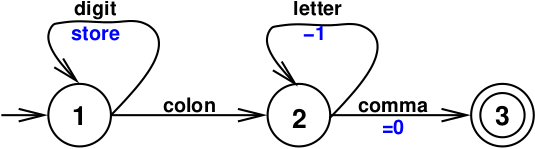
\includegraphics[width=0.6\linewidth]{fig/Calc-fsm-example-2.png}
    \caption{Basic functionality of a Calc-FSM for netstrings.}
    \label{fig:Calc-FSM}
\end{figure}\\\\
It is also important to mention that Grosch et al. established Calc-regular expressions based on the concept of regular expressions. For a much more in-depth explanation on Calc-regular languages and therefore the foundations of this thesis' work, we recommend reading the author's findings in their respective publication \cite{Calc-regular-paper}.
\subsection{Limitations of Calc-Regular Languages}
\label{2.3}
As already described above, Calc-regular languages define length-prefix languages with \textit{fixed} nesting.
This solid theoretical foundation describes the underlying problem really well but when looking at practical examples of length-prefix formats we can see its limitations. Most of the frequently used formats (\textit{e.g.} protobuf \cite{google-protobuf-encoding}, ASN.1 \cite{ASN.1}) employ \textit{variable} nesting and can therefore not be characterized by using Calc-regular languages. The distinction between \textit{fixed} and \textit{variable} nesting shall not be underestimated, as a formal definition for this type of languages is much more complex than it may sound at first. In this thesis we will present an extension to the aforementioned Calc-regular languages which shall ultimately be able to handle length-prefix languages using variable nesting.
In Grosch et al.'s paper \cite{Calc-regular-paper} they acknowledge the possibility for this extension and refer to it as 'Calc-context-free languages'. During our research, however, we have decided to name this extended language class 'Calc-LL(1)' instead.


\section{Calc-LL(1) Languages}
\label{3.0}
\subsection{Definition}
\label{3.1}
Informally, Calc-LL(1) languages can be described by looking at both Calc-regular languages as well as conventional LL(1) languages. LL(1) languages are a great instrument to guarantee a relatively simple and efficient parsing procedure. Calc-regular languages, on the other hand, provide us with the tools to represent languages using length-prefix format without variable nesting. Calc-LL(1) languages aim to merge the characteristics of these two language classes into a completely new class. This language class should then be able to parse length-prefix notation formats even with variable nesting, additionally employing the efficient, table-based parsing procedure that is given by LL(1).\\\\
As a matter of fact, many data serialization languages or formats currently in use that employ variable nesting are usually parsed using basic LL(1) parsing techniques and should therefore be classified as context-free. On a more detailed look, though, one can see inconsistencies that lead to these languages not actually being context-free as of Chomsky's strict definition \cite{Chomsky-Hierarchy}, as proven in theorem 2 in Grosch et al.'s paper \cite{Calc-regular-paper}.  This leads us to the conclusion that these languages form a separate, slightly different language class, which we establish and call Calc-LL(1).\\\\
As of this thesis, an exact formal definition of Calc-LL(1) languages has not yet been established. This thesis focuses on creating a working automaton model for Calc-LL(1) languages as well as presenting a grammar based on extended Backus-Naur form \cite{EBNF} that matches the definition from the automaton.
\subsection{Conventional LL(1)-Languages and Parsing Techniques}
\label{3.2}
An LL($k$) parser is a top-down parser for a subset of deterministic context-free languages. Subsequently, these parsers can be represented in a theoretical model by deterministic pushdown automatons. LL($k$) parsers parse from \textbf{L}eft to right and perform a \textbf{L}eftmost derivation of the input. Importantly, these parsers use $k$ tokens of look-ahead. This means that the parser can see at maximum $k$ of the upcoming tokens in the message to be parsed and decide their next step upon this knowledge \cite{Parsing-Techniques-(lookahead)}. LL(1) parsers therefore have a look-ahead of one token. They are the simplest form of LL($k)$ parsers and can parse LL(1) grammars respectively. Crucially, these LL(1) grammars are all deterministic.
\\\\
Parse tables are an important component of LL($k$) parsers due to the look-ahead. A parse table $M$ for any LL(1) grammar $G=\{N,\Sigma,P,S\}$\footnote{$N$ = non-terminal symbols, $\Sigma$ = terminal symbols, $P$ = productions, $S$ = starting non-terminal symbol.} is a two-dimensional table including all terminal symbols $\sigma \in \Sigma$ and all non-terminal symbols $A \in N$ as rows and columns respectively (or vice versa). Each table cell $m_{A,\sigma} \in M$ may either be empty or contain at most one production rule $p \in P$. Therefore, detecting if a grammar is LL(1) can be done by constructing the parse table. If every table cell has \textbf{at most} one entry, the grammar corresponding to the parse table is an LL(1) grammar. If a cell $m_{A,\sigma} \in M$ does contain some $p \in P$, this $p$ will mark the production rule that shall be executed next if the current non-terminal symbol on the stack is $A$ and the look-ahead token is $\sigma$. This table-parsed parsing guarantees determinism and additionally makes the procedure rather efficient, as the computation of the table can be done in advance and table-lookups are inexpensive. Also, since LL($k$) parsing can be carried out by a \textit{predictive recursive descent parser}\footnote{Predictive parsing is only possible for the class of LL($k$) grammars \cite{recursive-descent-parser}.} \cite{recursive-descent-parser}, backtracking is not required. This feeds into the efficiency of LL($k$) parsing, as parsing languages that require backtracking in recursive descent parsers may require exponential time \cite{recursive-descent-parser}. When the parser chooses one production in a parse table cell with regards to $A$ and $\sigma$, it knows with perfect certainty that this is the only possible production that can be executed in this situation. Therefore, the need for backtracking is eliminated.\\\\
All these properties make the LL(1) parsing technique a perfect fit for our purpose of parsing variably nested length-prefix languages. Of course, as this is a highly practical endeavour, the determinism trait is required. The look-ahead is also important for our cause, as we will see in more detail in chapter \hyperref[4.0]{4}. Without knowing about the upcoming token, the parser sometimes cannot make a deterministic decision when parsing some length-prefix formats. For more in-depth information about conventional parsing techniques, the book 'Parsing Techniques' \cite{Parsing-Techniques-2} by Grune and Jacobs is highly recommended.
\subsection{Calc-LL(1) Parsing and Split Parse Tables}
\label{3.3}
In a project at Bauhaus-Universität Weimar which was conducted prior to the research this thesis presents, a practical example of a Calc-LL(1) parser was implemented for netstrings. Also, a definition for so-called 'split parse tables' was introduced, specifically tailored for Calc-LL(1) languages. We will not go into detail much more about these findings, but they are publicly available on github in \cite{Calc-LL(1)-project}. The repository includes the parser for netstrings with detailed error-handling written in python, a generator for split parse tables for formal grammars also written in python and a report about these findings.


\section{Calc-PDA - An Automaton for Calc-LL(1) Languages}
\label{4.0}
\subsection{Introduction}
\label{4.1}
An extended definition of Calc-regular languages also requires an extended definition of Calc-FSMs. For Calc-regular languages a Calc-finite state machine is used as it is derived from regular languages where FSMs are also used. In an abstract perspective, an automaton model for Calc-LL(1) languages requires one more level of complexity than that of Calc-FSMs. When looking at Chomsky's hierarchy for formal languages \cite{Chomsky-Hierarchy}, pushdown automata (PDAs) are one level of complexity above finite state machines (FSMs). With this in mind, we define the Calc-pushdown automaton (Calc-PDA) as the automaton model for Calc-LL(1) languages.\\\\
To recap our core motivation, this automaton model should help with parsing length-delimited messages that can employ variable nesting. Messages that are formed correctly have to get parsed while messages that contain any sort of ill-formed features have to be rejected as soon as this malformation becomes clear to the machine. This includes detecting messages that are longer than the length-prefix intended, detecting malformed container structures, terminating correctly without compromising any bytes and many more cases.\\\\
As explained before in \hyperref[3.0]{3}, we only look at deterministic languages, therefore one could also say that we are defining a Calc-deterministic pushdown automaton (Calc-DPDA). In this thesis, however, we include the need for determinism in the core definition of our automaton so there is no difference in calling it Calc-DPDA or simply Calc-PDA. On the following pages, the process of creating the current\footnote{As of August, 2019.} iteration of the Calc-PDA definition for two example languages is explained in detail. These example languages are \hyperref[1.4]{netstrings} and \hyperref[1.5]{Google's protocol buffers (protobufs)}.

\subsection{Basic Components of Calc-PDAs}
\label{4.2}
When working with length-prefix languages and the respective Calc-PDA, one can see very quickly that the features employed in a regular PDA for context-free languages are not sufficient for the desired purpose. We not only want to parse these length-prefix messages, we also need to evaluate if the length-prefix value and the message's content length are equal or not. Therefore, we defined several additional properties for the Calc-PDA:
\begin{itemize}
    \item \textbf{Container-stack}\\This is a primitive stack which holds all integer values where each value represents the position of the whole message structure where a container ends. The topmost value gets popped from the stack each time the parser recognizes the end of a container's boundaries. This stack is necessary to allow for variably nested containers. The initial value on the stack is $\infty$.
    \item \textbf{Current position}\\This variable always holds one integer value. It is initialized with zero at the start of each message and incremented by one for each byte read during the parsing procedure. Therefore, this variable always represents the current byte position of the parser during the parsing procedure. The parser/Calc-PDA always needs to be aware of the current position to check for \textbf{each} byte, if the boundaries of an upper container have been exceeded. If this is the case, the length-prefix message is ill formed and the parsing of this message is terminated immediately.
    \item \textbf{Accumulator}\\The accumulator was also used in Calc-regular languages as explained in \hyperref[2.1]{2.1}. In the Calc-PDA definition, one accumulator is always active and behaves exactly as it does in the definition of Calc-regular languages. It can store bytes, transform them into a numerical representation to any base, and will then decrement its value by one for every content-byte read during parsing until it reaches zero.
    \item \textbf{Conditions}\\Logical conditions are the main factor for determining the next possible transition for the Calc-PDA. A condition always compares integer values using the \textit{current position}, the topmost symbol of the \textit{container stack} or an \textit{accumulator}.
    \item \textbf{Operations}\\An operation is basically a function which can be called at the end of any transition in a Calc-PDA. So far\footnotemark[6] there exist eight operations that are defined for the Calc-PDA:\\
    \begin{itemize}
        \item \texttt{store:} Takes the byte read during the transition and appends it to the string of bytes already stored in the accumulator.
        \item \texttt{toNum:} All bytes stored in the accumulator get evaluated in the order they were read and transformed into a numerical representation to any base (\textit{e.g.} decimal), the value remains in the accumulator as a single integer.
        \item \texttt{decr:} An integer value in the accumulator gets decremented by 1. This requires the accumulator to hold a valid integer.
        \item \texttt{reset:} The accumulator's contents get replaced with the empty string.
        \item \texttt{push($x$):} The integer value $x$ gets pushed onto the container stack. $x$ is always the value that had been stored inside the accumulator and has to be an integer, which means that the operation \texttt{toNum} must have been called prior to the \texttt{push} operation.
        \item \texttt{pop:} The topmost integer value gets popped from the container stack.
        \item \texttt{evaluateBytes($n$):} In the case of schema languages (\textit{e.g.} protobuf), type fields may contain important information about the nesting property of the underlying message. Therefore, the information in these type field bytes has to be evaluated. $n$ describes the amount of bytes that represent the type field. This operation can return the information extracted from these type field bytes to save them into variables\footnote{This feature will get clearer when discussing a Calc-PDA for protobufs in later chapters.}.
        \item \texttt{lookup($y$):} Also exclusively used for schema languages. If a type field does contain crucial information about the nesting properties, this operation determines whether an input $y$ taken from the operation \texttt{evaluateBytes($n$)} corresponds to either a single message or a container. It does so by looking through the given schema for this message. This operation returns either \textit{'string'} (for a single non-container message) or \textit{'container'} (for a message acting as a container). The output can then be used for a condition to determine which transition to execute next\footnotemark[7].
    \end{itemize}
\end{itemize}
It is important to mention, that contrary to a conventional PDA for context-free languages, Calc-PDAs choose the next transition based on two factors: The condition of a transition and its lookahead token (as described in \hyperref[3.1]{3}). Both these factors form a conjunction which has to be evaluated to true for a transition to fire.\\\\
On the following pages, some figures of automatons will get presented. In order to increase clarity, we use abbreviations for some features presented above: \texttt{'cp'} stands for the current position variable, \texttt{'stack'} describes the container stack, \texttt{'acc'} is the acronym for the accumulator and the \texttt{'stack-value'} represents the topmost value on the container stack. 
\subsection{A Calc-PDA for Netstrings}
\label{4.3}
\begin{figure}
    \centering
    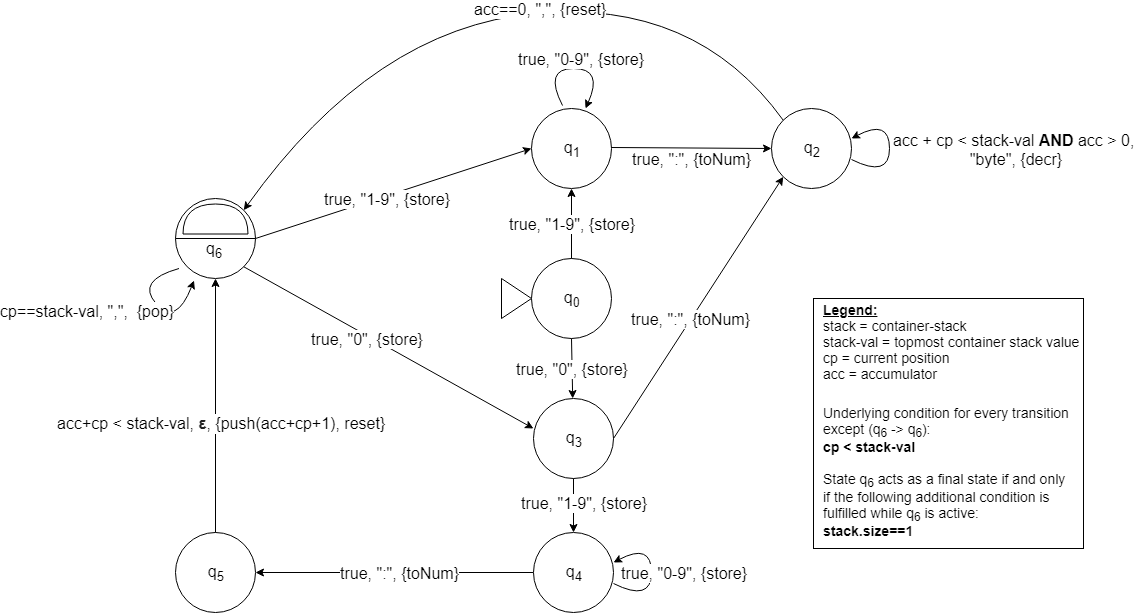
\includegraphics[width=\linewidth]{fig/Calc-PDA-netstrings-version_8.png}
    \caption{First iteration of a Calc-PDA specifically for netstrings.}
    \label{fig:fig-2-netstring-Calc-pda-1}
\end{figure}\hyperref[fig:fig-2-netstring-Calc-pda-1]{Figure 2} shows one of the first adoptions of a Calc-PDA specifically built for netstrings. This automaton is able to parse variably nested netstrings correctly, including the empty netstring \texttt{'0:,'}. Circles represent the states $\{q_0, q_1, q_2, q_3, q_4, q_5, q_6\}$ with $q_0$ being the initial state and $q_6$ a conditional accepting state. This means that $q_6$ only accepts when the condition '\texttt{stack.size==1}' is fulfilled while $q_6$ is active.
\begin{figure}
    \centering
    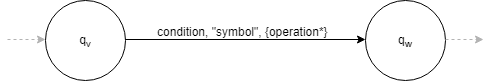
\includegraphics[width=0.8\linewidth]{fig/transitions-netstring-version_8.png}
    \caption{Transition structure of the Calc-PDA in \hyperref[fig:fig-2-netstring-Calc-pda-1]{Figure 2}}
    \label{fig:fig-3-transition-netstring-Calc-pda-1}
\end{figure}
In \hyperref[fig:fig-3-transition-netstring-Calc-pda-1]{Figure 3} we can see the basic structure of a transition in this Calc-PDA for netstrings. A transition from one state $q_v$ to another state $q_w$ always consists of:
\begin{itemize}
    \item a condition, which has to be true for the transition to be considered,
    \item the symbol, or byte in our case, that comes next and will be consumed by the transition. Hidden in this notation is the fact that the automaton has to evaluate the lookahead token (as described in \hyperref[3.2]{3.2}) at first. If the lookahead token is equal to the \textit{symbol}, it then continues executing the transition.
    \item The third component is a set of multiple operations where each operation is called sequentially in order.
\end{itemize}
In \hyperref[fig:fig-2-netstring-Calc-pda-1]{Figure 2} you can see that we have added an \textit{'underlying condition'} that reads \texttt{'stack-val $>$ cp'}, which is a condition that has to be true for every transition except for $q_6 \rightarrow q_6$. This condition checks before every transition, if the current position of the parser does not exceed the length defined by the length-prefix of the netstring. One could also add this condition to each transition except $q_6 \rightarrow q_6$ but for increased clarity we defined this in an underlying condition. \\\\
To understand this automaton more clearly, we will take a closer look at the procedure of processing netstrings with the Calc-PDA in \hyperref[fig:fig-2-netstring-Calc-pda-1]{Figure 2}.
We always start in the state $q_0$. This state will only be visited \textbf{once} at the beginning, highlighting the importance of the first length-prefix defining the outer size of the whole message in a variably nested netstring. When the next token in our lookahead is a digit $\in \{1,2,3,4,5,6,7,8,9\}$\footnote{In \hyperref[fig:fig-2-netstring-Calc-pda-1]{Figure 2} the notation "1-9" means that each digit from 1 up to 9 could be read. } and the underlying condition is true, the machine now proceeds to the state $q_1$ and starts processing a simple netstring not acting as a container. This is always done by visiting the states $q_1 \rightarrow q_2 \rightarrow q_6$ in that order.\\\\
While in $q_1$, the digits that form the length-prefix get read one by one and stored in the accumulator. If the lookahead-token equals a colon (\texttt{":"}) and the underlying condition still evaluates to true, the transition $q_1 \rightarrow q_2$ gets executed, the colon gets processed and the operation \texttt{toNum} gets called. This operation transforms the contents of the accumulator into the integer value defined in the length-prefix.\\\\
In state $q_2$, arguably the most important condition has to be evaluated. By checking if \texttt{'acc+cp $<$ stack-val'} equals true, the automaton can see if a nested netstring exceeds the upper container's size before any of the netstring's content bytes get read. \texttt{Stack-val} always represents the position in the whole netstring construct where the last container recognized by the parser ends. If the current position (\texttt{cp}) of the parser plus the length of the current netstring (\texttt{acc}) have a strictly lower value than the \texttt{stack-val}, the current netstring is within bounds of its corresponding container and the parsing may continue. In $q_2$, all content-bytes now get parsed one by one, decrementing the accumulator by one for every byte processed.
If the accumulator then equals zero (and the underlying condition still holds true), a comma (\texttt{","}) is expected and the transition $q_2 \rightarrow q_6$ gets executed. During this transition, the accumulator's contents get replaced by the empty string due to the operation \texttt{reset}.\\\\
In state $q_6$, the machine first checks if the size of the container stack equals one. If this is the case, it accepts since all containers have been completed and parsed successfully. Keep in mind, that the initial value always remains on the stack, which is why we accept at a stack size of one instead of zero. Should the stack be of size greater than one, the automaton can execute three possible transitions:
\begin{itemize}
    \item If the condition \texttt{'cp==stack-val'} holds true, a comma (\texttt{","}) is expected, processed and the topmost value on the container stack (\texttt{stack-val)} gets popped and discarded. This transition leads back to $q_6$ and, in practice, finalizes the parsing procedure for a container.
    \item If the underlying condition \texttt{'cp < stack-val'} holds true and the lookahead equals a digit $\in \{1,2,3,4,5,6,7,8,9\}$, the machine recognizes another simple non-container netstring and proceeds to state $q_1$.
    \item If the underlying condition holds true and the lookahead equals a zero, the automaton recognizes a netstring representing a container and proceeds to state $q_3$.
\end{itemize}
If the first digit of the length-prefix is zero, the automaton always ends up in state $q_3$. From here on, the fringe case of the empty netstring can be detected: if the lookahead is equal to a colon (\texttt{":"}) and not a digit, transition $q_3 \rightarrow q_2$ is executed. Otherwise, should the lookahead contain a digit from zero to nine, a container is recognized and transition $q_3 \rightarrow q_4$ gets called.\\\\
In $q_4$, digits get read one by one and stored in the accumulator and if the lookahead contains a colon (\texttt{":"}), the accumulators values get evaluated to an integer number by calling \texttt{toNum} during $q_4 \rightarrow q_5$.\\\\
Then, for the transition $q_5 \rightarrow q_6$ to execute, the condition \texttt{'acc+cp < stack-val'} has to hold true to make sure that the newly read netstring container does not exceed any container that it is contained in. If this condition is validated, the integer value \texttt{'acc+cp+1'} is pushed onto the container stack. This value represents the position where this specific container ends in the entire netstring structure that is currently processed by the machine.\\\\
As a side note, this machine can easily be transformed into one that accepts netstrings that do not use the end-of-content comma. By just removing the comma from transitions $q_2 \rightarrow q_6$ and $q_6 \rightarrow q_6$, this can be achieved rather easily. This also shows that the comma in the original netstring definition does not serve any purpose other than to increase human readability. Arguably, though, human readability really does not have to be guaranteed in data serialization.


\subsection{Parsing Procedure for Netstring Examples}
\label{4.4}
To strengthen the understanding of the machine's procedure, we will present several examples of netstrings being processed by the Calc-PDA for netstrings. Tables \hyperref[tab:tab1-netstring-1-Calc-pda-state-sequence]{1}, \hyperref[tab:tab2-netstring-2-Calc-pda-state-sequence]{2}, \hyperref[tab:tab3-netstring-3-Calc-pda-state-sequence]{3} and \hyperref[tab:tab4-netstring-4-Calc-pda-state-sequence]{4} list the sequence of states visited during the processing of the corresponding netstring. $q_i$ with $i \in \{0,1,2,3,4,5,6\}$ represents a state, the arrow ($\rightarrow$) highlights a transition between two states and the symbol below each arrow signals the current symbol of the netstring being parsed or the operation being performed during that transition. In the end we either accept in $q_6$ if there is only  the initial value on stack or we reject if this accepting condition does not hold while in $q_6$ or if in any other state, no more transitions can be fired. The reader may go through the automaton step by step and validate their choices by looking at the given sequence. We will list four examples below, although, in practice, there are many more cases where the automaton parses correctly and recognizes errors and malformed netstrings.\\
\begin{table}
    \centering
    \begin{tabular}{|lllllllllll|}\hline
         $\rightarrow q_0$ &$\rightarrow q_3$ & $\rightarrow q_4$ & $\rightarrow q_4$ & $\rightarrow q_5$ & $\rightarrow q_6$ & $\rightarrow q_1$ & $\rightarrow q_2$ & $\rightarrow q_2$ & $\rightarrow q_2$ & $\rightarrow q_2$  \\
        & \texttt{0} &\texttt{2} &\texttt{0} &\texttt{:} & \tiny{push(20+4)} & \texttt{5}&\texttt{:} & \texttt{H} & \texttt{e} & \texttt{l}\\[10pt]\hline
        $\rightarrow q_2$ &$\rightarrow q_2$ &$\rightarrow q_6$ &$\rightarrow q_3$&$\rightarrow q_4$ &$\rightarrow q_5$ &$\rightarrow q_6$ &$\rightarrow q_1$ &$\rightarrow q_2$ &$\rightarrow q_2$ &$\rightarrow q_2$\\
         \texttt{l} & \texttt{o} & \texttt{,} & \texttt{0} & \texttt{8} & \texttt{:}& \tiny{push(8+15)} & \texttt{5}& \texttt{:}& \texttt{W} & \texttt{o} \\[10pt]\hline
        $\rightarrow q_2$ &$\rightarrow q_2$ &$\rightarrow q_2$ &$\rightarrow q_6$ &$\rightarrow q_6$ &$\rightarrow q_6$ &$\rightarrow q_6$ &$\rightarrow q_6$ & $\rightarrow$ \tiny{accept} & & \\
        \texttt{r} & \texttt{l} & \texttt{d} & \texttt{,} & \tiny{pop} & \texttt{,}& \tiny{pop} & \texttt{,}  &  & \\[10pt]\hline
    \end{tabular}
    \caption{Calc-PDA state sequence for the netstring '\texttt{020:5:Hello,08:5:World,,,}'.}
    \label{tab:tab1-netstring-1-Calc-pda-state-sequence}
\end{table}
\\\hyperref[tab:tab1-netstring-1-Calc-pda-state-sequence]{Table 1} highlights the parsing of the well-formed netstring '\texttt{020:5:Hello,08:5:World,,,}' where the machine correctly accepts in the end.\\
\begin{table}
    \centering
    \begin{tabular}{|llllll|}\hline
         $\rightarrow q_0$ &$\rightarrow q_3$ & $\rightarrow q_4$ & $\rightarrow q_5$ & $\rightarrow q_6$ & $\rightarrow$ \tiny{reject}\\
        & \texttt{0} &\texttt{7} &\texttt{:} &\tiny{push(7+4)} &   \\[10pt]\hline
    \end{tabular}
    \caption{Calc-PDA state sequence for the message '\texttt{07:Testing,}'.}
    \label{tab:tab2-netstring-2-Calc-pda-state-sequence}
\end{table}
\\\hyperref[tab:tab2-netstring-2-Calc-pda-state-sequence]{Table 2} highlights the malformed netstring '\texttt{07:Testing,}'. The first length-prefix indicates a container but the content does not resemble another netstring with a length-prefix, which would be required. Instead it only contains a simple string. This netstring gets rejected eventually in $q_6$, when the look-ahead token can not be recognized as either \texttt{"1-9"} or \texttt{"0"} and the accepting condition (\texttt{stack.size==1)} is not met. Keep in mind that the only error in this netstring is the leading zero at the beginning of the length-prefix, as this indicates a container. By removing this zero, one would have a perfectly fine (non-nested) netstring.\\
\begin{table}
    \centering
    \begin{tabular}{|lllllllllll|}\hline
         $\rightarrow q_0$ & $\rightarrow q_3$ & $\rightarrow q_4$ & $\rightarrow q_4$ & $\rightarrow q_5$ & $\rightarrow q_6$ &$\rightarrow q_1$ & $\rightarrow q_2$ & $\rightarrow q_2$ & $\rightarrow q_2$ & $\rightarrow q_2$\\
        &\texttt{0}&\texttt{1}&\texttt{1}&\texttt{:}&\tiny{push(11+6)}& \texttt{5} &\texttt{:} &\texttt{T} & \texttt{o} & \texttt{o}\\[10pt]\hline
         $\rightarrow q_2$ &$\rightarrow$ \tiny{reject} & & & & & & & & &\\
         \texttt{l} & \texttt{o} & & & & & & & & &\\[10pt]\hline
    \end{tabular}
    \caption{Calc-PDA state sequence for the message '\texttt{011:5:Toolong,,}'.}
    \label{tab:tab3-netstring-3-Calc-pda-state-sequence}
\end{table}
\\\hyperref[tab:tab3-netstring-3-Calc-pda-state-sequence]{Table 3} represents the parsing procedure of the malformed netstring '\texttt{011:5:Toolong,,}'. Here, the size of the contents of the inner, nested netstring exceed the declared length-prefix. Therefore, the parsing has to stop immediately after the fifth content byte of the inner netstring has been read, as this is the point where the parser notices the error and prevents additional bytes to be compromised.\\
\begin{table}
    \centering
    \begin{tabular}{|lllllllllll|}\hline
         $\rightarrow q_0$ &$\rightarrow q_1$ & $\rightarrow q_2$ & $\rightarrow q_2$ & $\rightarrow q_2$ & $\rightarrow q_2$ & $\rightarrow q_6$ & $\rightarrow$ \tiny{accept} & & &\\
        & \texttt{3} &\texttt{:} &\texttt{a} & \texttt{b} & \texttt{c} & \texttt{,} & & & &\\[10pt]\hline
    \end{tabular}
    \caption{Calc-PDA state sequence for the message '\texttt{3:abc,xyz}'.}
    \label{tab:tab4-netstring-4-Calc-pda-state-sequence}
\end{table}
\\Finally, \hyperref[tab:tab4-netstring-4-Calc-pda-state-sequence]{Table 4} shows the parsing behaviour of the Calc-PDA for the example string'\texttt{3:abc,xyz}' and therefore the behaviour when appending arbitrary symbols behind its end-of-content symbol (\texttt{','}). The parsing correctly stops after the comma has been read, as the accepting condition that the container stack's size is equal to one is met while the machine is in state $q_6$. This accepts the netstring and the following symbols '\texttt{xyz}' do not get considered. In practice, these additional symbols could be used as some sort of padding.

\subsection{Guaranteeing Determinism in Calc-PDAs}
\label{4.5}
As mentioned in earlier chapters, the Calc-PDA has to be deterministic in all steps. A nondeterministic approach does not yield much practical use, especially not when considering data serialization where we operate on a low level of computational complexity. When examining the Calc-PDA for netstrings in \hyperref[fig:fig-2-netstring-Calc-pda-1]{Figure 2}, we can see that there is one transition $(q_5 \rightarrow q_6)$ that is different from other transitions. It does not read or process a symbol, we have replaced it with an $\varepsilon$ instead. This is a crucial transition, as it represents a step from a potential parser where it does \underline{not} process an input symbol and therefore also a step where the current position of the parser does not change. This characteristic is due to the necessary sequential execution of some operations and conditions that depend on each other. The accumulators contents have to be converted to a numerical representation by calling the operation \texttt{toNum} in transition $(q_4 \rightarrow q_5)$ before the condition in $(q_5 \rightarrow q_6)$ can use this accumulator value to check if \texttt{'acc+cp $<$ stack-val'} equals true.\\\\
The structure of a Calc-PDA transition in mind, we can now formulate exact requirements for such a transition to be valid in a Calc-PDA:
\begin{itemize}
    \item Trivially, a state $q_v$ where the transition starts and a state $q_w$ where it ends have to be known ($q_v \rightarrow q_w$),
    \item a condition $c$ which can be any logical conjunction as described in \hyperref[4.3]{4.3},
    \item optionally, a lookahead-token $z$. This is not necessarily required as discussed earlier in this chapter when looking at transition $q_5 \rightarrow q_6$.
    \item a finite set $O$ of valid Calc-PDA operations.
\end{itemize}
A transition in the Calc-PDA, which is deterministic by definition, is only valid if with the inputs $q_v,c,z$, there exists at maximum one possible $q_w$ that can be reached.\\\\
As this can be rather unintuitive to grasp, we were prompted to search for a more exact visual representation of transitions in the Calc-PDA. Eventually, we decided to partition each transition into three subparts: The condition, the symbol read, and the set of operations performed. This ultimately leads to a Calc-PDA for netstrings as seen in \hyperref[fig:fig-4-netstring-Calc-pda-2]{Figure 4}.
\begin{figure}
    \centering
    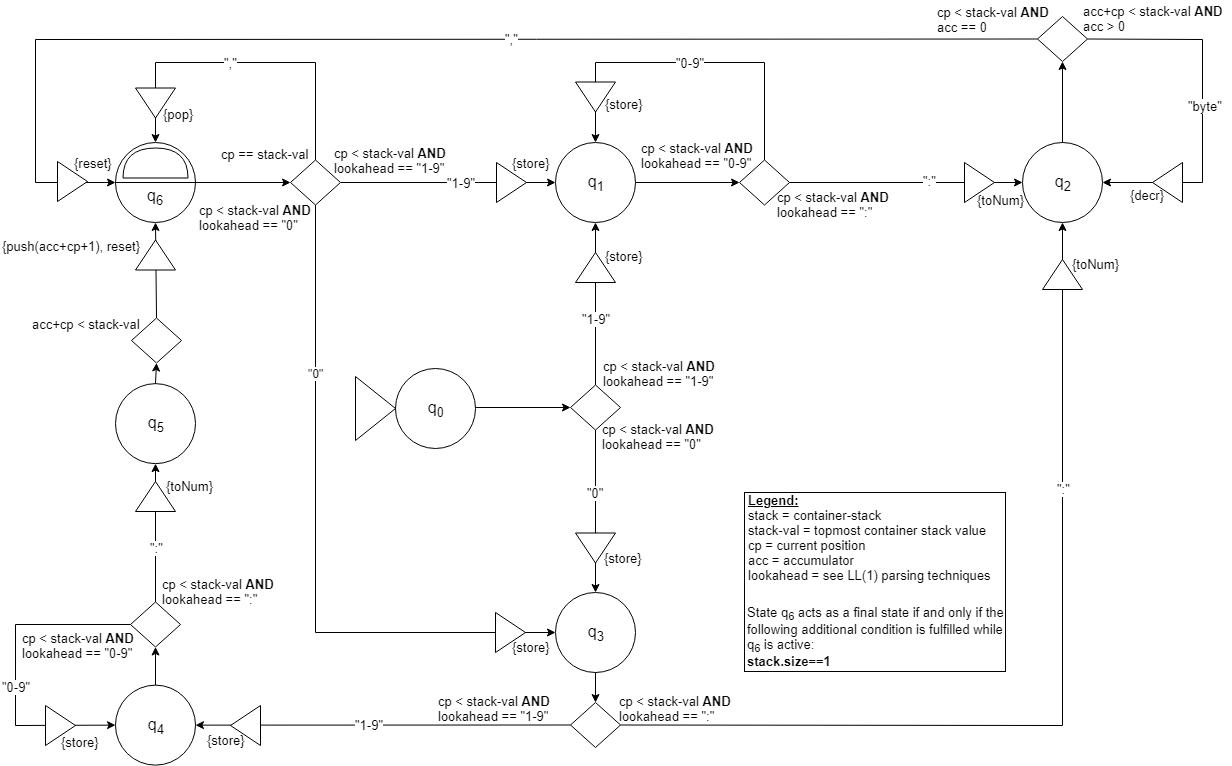
\includegraphics[width=\linewidth]{fig/Calc-PDA-netstrings-version_10.png}
    \caption{Final iteration of a Calc-PDA specifically for netstrings.}
    \label{fig:fig-4-netstring-Calc-pda-2}
\end{figure}
While this automaton looks much more complex than the one in \hyperref[fig:fig-2-netstring-Calc-pda-1]{Figure 2}, they are both equal. Importantly, though, this reworked automaton has more of the core definitions embedded visually. While the look-ahead was not specifically mentioned in the conditions of the first iteration, it is now properly included. The 'underlying condition' which was introduced in the first version has also been moved to the respective transitions.
\begin{figure}
    \centering
    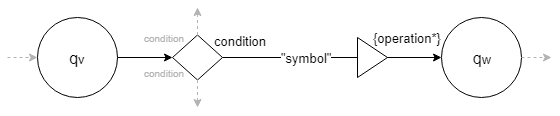
\includegraphics[width=0.8\linewidth]{fig/transitions-netstring-version_10.png}
    \caption{Transition structure of the Calc-PDA in \hyperref[fig:fig-4-netstring-Calc-pda-2]{Figure 4}.}
    \label{fig:fig-5-transition-netstring-Calc-pda-2}
\end{figure}\\\\
The structure of such a newly defined transition from one state $q_v$ to another state $q_w$ can be seen in \hyperref[fig:fig-5-transition-netstring-Calc-pda-2]{Figure 5}. Conditions are now represented by diamonds where each condition-diamond may only have one input-arrow from states (circles) exclusively. These condition-diamonds can have more than one outgoing arrow, representing the power of these condition that enables them to make deterministic decisions. In other words, each condition-diamond can evaluate which state should be reached next based on several possible conditions. These conditions $c_1,c_2,...,c_n$ have to be distinct from each other, meaning $c_i \wedge c_j = \texttt{false}$  $\forall i,j = \{1,2...,n\}$ and $i\neq j$. In practice, the maximum conditions per diamond we used was three in the condition-diamond for state $q_6$. In theory, though, each condition-diamond can have an arbitrary number of conditions, as long as they fulfill their requirements.\\\\
After each branch coming from a condition-diamond, a symbol may be read although it is not required (as seen in state $q_5\rightarrow q_6$). Subsequently, if a symbol (or byte) is read, the current position value also gets incremented by one. Finally, before state $q_w$ is reached where the transition converges to, all operations performed are listed in curly brackets notating a set. By adding a triangle just before the end of the transition, we represent the set of operations as the third subpart of a transition\footnote{One could redefine the initial triangle used to represent the starting state $q_0$ as an operation triangle with an operation \texttt{initialize} to be consistent with the definition.}.
\subsection{A Calc-PDA for Protobufs}
\label{4.6}
\begin{figure}
    \centering
    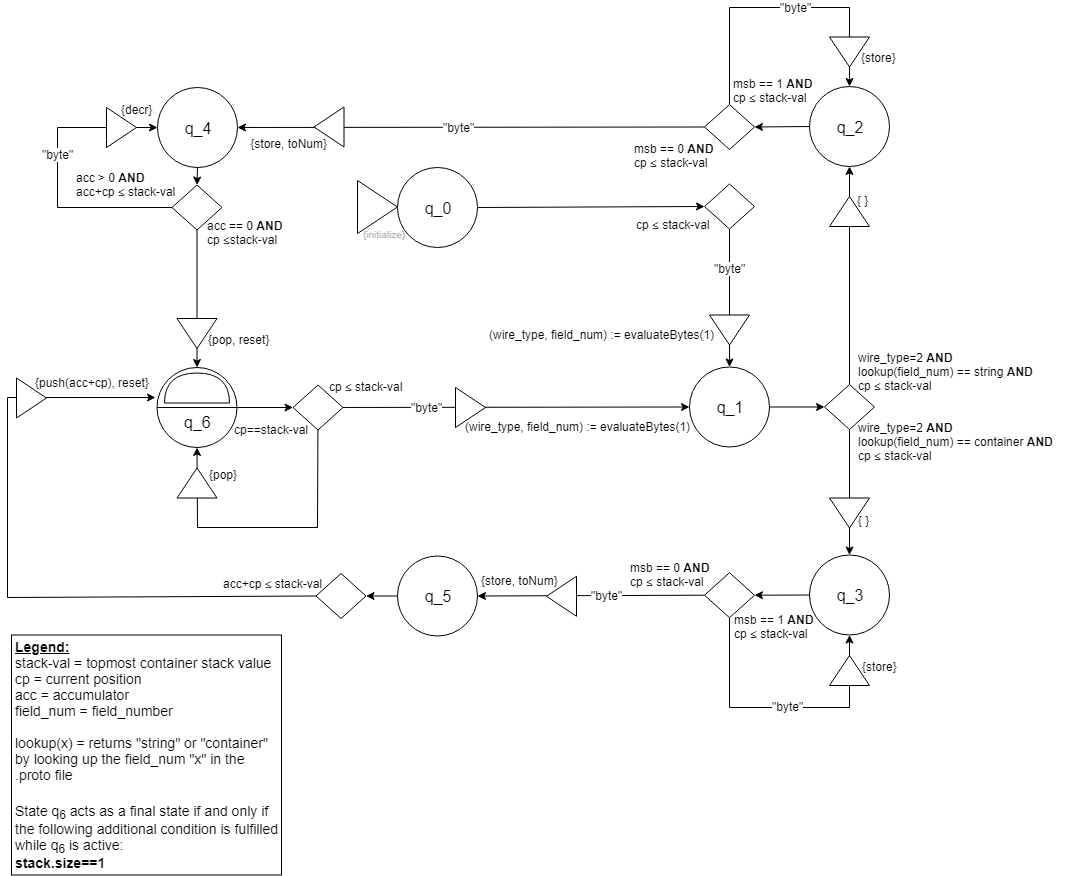
\includegraphics[width=\linewidth]{fig/Calc-protobuf-PDA-version-7-notitle.png}
    \caption{Calc-PDA specifically for Google protocol buffers.}
    \label{fig:fig-6-protobuf-Calc-pda-1}
\end{figure}
Netstrings are the representative for one form of length-prefix formats used. The next representative, which is also more commonly used in practice, represents another form of length-prefix languages. Whereas netstrings employ certain delimiters which are staples in each instance (such as the colon after each length-prefix and the comma as and end-of-content symbol), Google protocol buffers (protobufs) do not include such symbols. In protobufs, the first length byte follows immediately after the last type byte, and the first content byte follows immediately after the last length byte.\\\\ In \hyperref[fig:fig-6-protobuf-Calc-pda-1]{Figure 6} we can see a Calc-PDA for protobufs. The core functionality, of course, remains the same, using container-stack, accumulator, etc. As already defined in \hyperref[4.2]{4.2}, this Calc-PDA uses two additional operations which are crucial to length-prefix languages that convey nesting-information in their type fields and schema files. Protobufs specifically include two variables in their type fields: \texttt{'wire type'} and \texttt{'field number'}. The wire type mainly discloses the type of message and what it is used for. We focus on \texttt{wire type = 2}, as this defines a length-delimited message that can represent either strings, embedded messages or packed repeated fields \cite{google-protobuf-wire-type}. There exist five wire types in total, each marking slightly different properties. For example, wire type 1 represents only 64 bit blocks, which therefore do not have to employ length fields. The Calc-PDA does allow the extension to consider all wire types by branching out in the condition-diamond after state $q_1$. At this decision point, the wire type is important to decide which transition to consider next. \\\\Looking at messages of wire type 2, however, the \texttt{field number} of a message is linked to the schema file with the ending \texttt{.proto} which protobuf uses. This field number is important for us, as there is no way to determine if a message acts as a single string or as a container by just looking at the byte encoding. This crucial information can be extracted by searching for the \texttt{field number}, which is unique for each protobuf structure, in the corresponding \texttt{.proto} schema file. From there we can extract if a message acts as a single string or a container. In the Calc-PDA, we extract the \texttt{wire\_type} and \texttt{field\_num} by calling the operation \texttt{evaluateBytes} on the type byte which includes both these numbers. By employing the operation \texttt{lookup(field\_num)}, the \texttt{field number} is looked up in the schema file and either \texttt{'string'} or \texttt{'container'} is returned respectively. We use this output to evaluate conditions in the condition-diamond following state $q_1$. We treat these operations \texttt{evaluateBytes}, \texttt{lookup}, as well as the operation \texttt{toNum} as oracle operations, which always return the correct output we need. We do not specify their exact functionality in detail, as this would exceed the current scope of our research. From our perspective, though, these operations should be able to be implemented rather easily.\\\\
As protobuf does not include a symbol which marks the end of the length field, the end of a variably sized length field has to be signaled otherwise. Therefor, protobuf uses so-called 'varints' to represent integer values in its length field. Each byte in a varint, except for the last one, has the most signficant bit set. Therefore, by detecting that the most significant bit has been set to zero in a byte, one can determine that this is the last byte in the length field. The last seven bits from each byte are used to store the binary representation of the integer in groups of seven bits with the least significant group first \cite{google-protobuf-varints}. The usage of varints is the reason why after states $q_2$ and $q_3$ we check for the most significant bit (msb) being either 0 or 1 to determine when to stop parsing the length field. If \texttt{msb==1}, the automaton keeps parsing bytes and adds those values to the accumulator. If \texttt{msb==0}, however, the machine stores the last byte in the accumulator, evaluates its contents and proceeds to the next state $q_4$ or $q_5$ respectively.

\subsection{Parsing Procedure for Protobuf Examples}
\label{4.7}
Just as presented in \hyperref[4.4]{4.4} for netstrings, Tables \hyperref[tab:tab5-protobuf-1-Calc-pda-state-sequence]{5} and \hyperref[tab:tab6-protobuf-2-Calc-pda-state-sequence]{6} show examples of protobuf-messages being processed by the corresponding Calc-PDA for protobufs in \hyperref[fig:fig-6-protobuf-Calc-pda-1]{Figure 6}. Again, $q_i$ with $i\in\{0,1,2,3,4,5,6\}$ represents a state, the arrow($\rightarrow$) highlights a transition between two states and the symbol below each arrow signals the current symbol of the netstring being parsed or the operation being performed during that transition. In the end we either accept or reject.\\
\begin{table}
    \centering
    \begin{tabular}{|lllllllllll|}\hline
         $\rightarrow q_0$ &$\rightarrow q_1$ & $\rightarrow q_3$ & $\rightarrow q_5$ & $\rightarrow q_6$ & $\rightarrow q_1$ & $\rightarrow q_3$ & $\rightarrow q_5$ & $\rightarrow q_6$ & $\rightarrow q_1$ & $\rightarrow q_2$\\
        & \texttt{0A} &\tiny{container} &\texttt{12} & \tiny{push(18+2)} & \texttt{12} & \tiny{container} & \texttt{07} & \tiny{push(7+4)} & \texttt{1A} & \tiny{string} \\[10pt]\hline
        $\rightarrow q_4$ &$\rightarrow q_4$ & $\rightarrow q_4$ & $\rightarrow q_4$ & $\rightarrow q_4$ & $\rightarrow q_4$ & $\rightarrow q_6$ & $\rightarrow q_1$ & $\rightarrow q_2$ & $\rightarrow q_4$ & $\rightarrow q_4$\\
        \texttt{05} &\texttt{53} &\texttt{68} & \texttt{6F} & \texttt{72} & \texttt{74} & \tiny{pop} & \texttt{22} & \tiny{string} & \texttt{07}& \texttt{45} \\[10pt]\hline
        $\rightarrow q_4$ &$\rightarrow q_4$ & $\rightarrow q_4$ & $\rightarrow q_4$ & $\rightarrow q_4$ & $\rightarrow q_4$ & $\rightarrow q_6$ & $\rightarrow$ \tiny{accept} & & & \\
        \texttt{78} &\texttt{61} &\texttt{6D} & \texttt{70} & \texttt{6C} & \texttt{65} & \tiny{pop} &  &  & & \\[10pt]\hline
    \end{tabular}
    \caption{Calc-PDA state sequence for the protobuf-message '\texttt{0A 12 12 07 1A 05 53 68 6F 72 74 22 07 45 78 61 6D 70 6C 65}'.}
    \label{tab:tab5-protobuf-1-Calc-pda-state-sequence}
\end{table}
\\Our first example will be a correctly formed protobuf-message. The structure of this message can be depicted as follows: "\texttt{container$_1$\{container$_2$\{string$_1$\}string$_2$\}}". \texttt{Container$_1$} holds a concatenation of another \texttt{container$_2$} and some \texttt{string$_2$}. The inner \texttt{container$_2$} also contains a \texttt{string$_1$}. In this case, we set \texttt{string$_1$} to '\texttt{Short}', and \texttt{string$_2$} to '\texttt{Example}'. Therefore, the structure of this protobuf-message looks like this: 
\begin{center}
    \texttt{$T_{c1}$ 18 $T_{c2}$ 7 $T_{s1}$ 5 S h o r t $T_{s2}$ E x a m p l e}
\end{center} with $T_{c1}$, $T_{c2}$ as the type fields for each container and $T_{s1}$, $T_{s2}$ as type fields for each string respectively always followed by their corresponding length field. As we do need a byte representation of this message, we will convert this message into bytes with hexadecimal representation:
\begin{center}
    \texttt{0A 12 12 07 1A 05 53 68 6F 72 74 22 07 45 78 61 6D 70 6C 65}
\end{center}
We have set $T_{c1}$ to the byte '\texttt{0A}', meaning that \texttt{container$_1$}'s \textit{field number} equals 1 and their \textit{wire type} equals 2. For $T_{c2}, T_{s1}, T_{s2}$ the wire type is always 2, and we set their field numbers as follows: $T_{c2} \Rightarrow 2, T_{s1} \Rightarrow 3, T_{s2} \Rightarrow 4$. Keep in mind that each protobuf-message has to have a schema file (\texttt{.proto}-file). In this case, we omit creating such a file and simply define that the corresponding schema file marks field numbers 1 and 2 as containers and field numbers 3 and 4 as simple strings. \hyperref[tab:tab5-protobuf-1-Calc-pda-state-sequence]{Table 5} shows the parsing procedure of this message using the Calc-PDA for protobufs.\\
\begin{table}
    \centering
    \begin{tabular}{|lllllllllll|}\hline
         $\rightarrow q_0$ &$\rightarrow q_1$ & $\rightarrow q_3$ & $\rightarrow q_5$ & $\rightarrow q_6$ & $\rightarrow q_1$ & $\rightarrow q_2$ & $\rightarrow q_4$ & $\rightarrow$ \tiny{reject} & & \\
        & \texttt{2A} &\tiny{container} &\texttt{04} & \tiny{push(4+2)} & \texttt{32} & \tiny{string} & \texttt{07} & \texttt{74} &  & \\[10pt]\hline
    \end{tabular}
    \caption{Calc-PDA state sequence for the message '\texttt{2A 04 32 07 74 6F 6F 6C 6F 6E 67}'.}
    \label{tab:tab6-protobuf-2-Calc-pda-state-sequence}
\end{table}
\\The second message example is the protobuf-like message '\texttt{2A 04 32 07 74 6F 6F 6C 6F 6E 67}' with the structure \texttt{container$_1$\{string$_1$\}}. In this case, the length-prefixes for \texttt{container$_1$} and \texttt{string$_1$} are "\texttt{04}" and "\texttt{07}" respectively and the content of \texttt{string$_1$} is the text "\texttt{Toolong}". 
\begin{center}
    \texttt{$T_{c1}$ 4 $T_{s1}$ 7 T o o l o n g}
\end{center}
In this case, $T_{c1}$, the type field for \texttt{container$_1$} contains the wire type 2 and the field number 5, which corresponds to a container in the schema file. $T_{s1}$, the type field for \texttt{string$_1$} contains the wire type 2 and the field number 6 associated with a string in the schema file.
Since the length-prefix for \texttt{container$_1$} only reads 4 (in decimal representation) but \texttt{string$_1$} is much longer than 4 bytes, this is not a valid protobuf message. In \hyperref[tab:tab6-protobuf-2-Calc-pda-state-sequence]{Table 6} you can see that the Calc-PDA parses this string correctly and terminates as soon as it detects this flaw, right after reading the length field of \texttt{string$_1$}. As \texttt{string$_1$}'s length field equals 7, the necessary condition '\texttt{acc+cp $\leq$ stack-val}' does not hold, as '\texttt{7+4 $\nleq$ 6}'. With this condition evaluating to false, no more transition can be executed and the machine rejects the input.
\subsection{Condensed, Formal Definition for Calc-PDAs}
\label{4.8}
We define a Calc-PDA as a deterministic automaton $M=(Q,\Sigma,\Gamma, \delta, q_0,Z,q_f)$:
\begin{description}
    \item[$Q$] is a finite set of states $q_0, q_2,...q_n$ with $n = |Q|-1$.
    \item[$\Sigma$] is the input alphabet. In the case of data serialization: $\Sigma =$ all possible bytes.
    \item[$\Gamma$] $=\mathbb{N}$ is the container stack alphabet.
    \item[$\delta$] $\in Q \times C \times \Sigma\cup\varepsilon \times O \times Q$ is the transition relation, where $C$ is a conjunction of $1,2,...n$ \textit{conditions} $c_i$ with $C=c_1 \land c_j \land ... \land c_n \ |\ 1 \leq j \leq n$ and $O$ is a finite set of \textit{operations}\footnote{$O$ can also be the empty set.}.
    \item[$q_0$] $\in Q$ is the starting state.
    \item[$Z$] $\in \Gamma\cup\infty$ is the initial stack symbol (in theory, always $Z=\infty$).
    \item[$q_f$] $\in Q$ is the accepting state. This state only accepts when the condition \texttt{'stack.size==1'} is met while $q_f$ is active.
\end{description}
\textbf{Unique features in Calc-PDAs} (as explained in \hyperref[4.2]{4.2})\textbf{:}
\begin{itemize}
    \item Container stack
    \item Current position
    \item Accumulator
    \item Conditions
    \item Operations
\end{itemize}\vspace{10pt}
\textbf{The set of \textit{conditions}:}
\begin{itemize}
    \item \texttt{'cp$<$stack-val'}
    \item \texttt{'cp$\leq$stack-val'}
    \item \texttt{'acc+cp$<$stack-val'}
    \item \texttt{'acc+cp$\leq$stack-val'}
    \item \texttt{'cp$==$stack-val'}
    \item \texttt{'acc$>$0'}
    \item \texttt{'acc$==$0'}
    \item \texttt{'lookahead$==x$'}
    \item \texttt{'stack.size$==$1'}
\end{itemize}
\vspace{10pt}
\textbf{The set of \textit{operations}:}
\begin{itemize}
    \item \texttt{'store'}
    \item \texttt{'toNum'}
    \item \texttt{'decr'}
    \item \texttt{'reset'}
    \item \texttt{'push($x$)'}
    \item \texttt{'pop'}
    \item \texttt{'}$int\big[$ $\big]$ \texttt{evaluateBytes($n$)'}
    \item \texttt{'}$string$ \texttt{lookup($y$)'}
\end{itemize}

\subsection{The importance of the initial stack symbol $Z$}
For the initial stack symbol $Z$, we generally use $\infty$ in our theoretical models, signaling that the value of the first length-prefix read by the machine can be of any size. This is obviously not applicable in practical use, as length-prefix messages with unlimited length can neither be detected nor handled by finite computers. In practice, therefore, choosing values other than $\infty$ for $Z$ can be very helpful for establishing length limits for messages. The first length-prefix of any message structure always defines the size of the complete message and is regulated by the initial stack value.\\\\ This works since the conditions that check if some nested structure would exceed its upper container, \texttt{'acc+cp < stack-val'} for netstrings or \texttt{'acc+cp $\leq$ stack-val'} for protobufs, will always use the initial stack-value for comparison in the first iteration of the machine. If this value is exceeded by \texttt{'acc+cp'}, the parsing procedure will terminate immediately. One could therefore also see the initial stack value $Z$ as some sort of invisible container with a constant size $Z$, where each message is included in such a container and can therefore not exceed their length $Z$.


\section{EBNF-like Grammars for Calc-LL(1) Languages}
\label{5.0}
\subsection{Differences to conventional formal grammars}
\label{5.1}
In this chapter, we want to lay some groundwork on the creation of grammars for Calc-LL(1) languages. We will use the conventional notation of Extended Backus-Naur form (EBNF) \cite{EBNF} with additional features distinct to Calc-LL(1) languages. As shown throughout \hyperref[4.0]{chapter 4}, conditions and operations are a vital part of the Calc-LL(1) concept. Therefore, these tools also have to be implemented in our 'Calc-EBNF' to guarantee a correct grammar which is equivalent to the corresponding Calc-PDA. In sections \hyperref[5.2]{5.2} and \hyperref[5.3]{5.3}, propositions for Calc-EBNFs for netstrings and protobufs are made to show how these grammars could look like.\\\\
Before examining these examples, though, some explanations have to be made:
\begin{itemize}
    \item Due to us working on the binary level of data serialization, there are only two terminal symbols representing bits: 0 and 1,
    \item the denomination $\{0,1\}^n$ refers to a sequence of bits of length $n$,
    \item the denomination '\texttt{T}$^n$' with \texttt{T} being a non-terminal refers to a concatenation of these non-terminals where the \textbf{total length measured in terminal symbols} of \texttt{T} is of length $n$.
    \item The current position is called '\texttt{cp}' and is incremented by 1 for each \textbf{eight} terminal symbols read (as we are looking at bytes which consist of eight bits each), the topmost value on the container stack is called '\texttt{stack-val}'.
    \item The notation '[$\ell\leftarrow$]\texttt{A}' means, that some function is called which converts the value of the non-terminal \texttt{A} into a numeric value which is then allocated to the variable $\ell$. As our non-terminals are either 0 or 1, each non-terminal will eventually be broken down to a sequence of bits \{$0,1$\}$^m$, which can easily be used to determine the value of $\ell$ with $\ell < 2^m$.\\$E.g.$, '[$\ell\leftarrow$]\texttt{length}' saves the numeric value from the length field into the variable '$\ell$' for further use.
    \item the operations \texttt{push(x)}, \texttt{pop} and \texttt{lookup(y)}\footnote{These operations work just as explained in \hyperref[4.2]{4.2}.} are included in Calc-EBNFs.
    Each operation is embedded in square brackets and can be described as behaving similarly to a non-terminal, as each operation executes as soon as it is called and is the lowest unit in Calc-EBNFs.
    \item By writing '\texttt{B[$\rightarrow$(u,v,w)]}', the variables \texttt{u}, \texttt{v} and \texttt{w} are given as parameters to the non-terminal \texttt{B}.
    \item A non-terminal \texttt{B} can use parameters to decide which right-side production rule to choose from. These parameters can be evaluated to logical statements producing a boolean value. As our grammar has to be deterministic, both statements can never output the same boolean value with the same inputs. The evaluation of the non-terminal \texttt{B} to some right-hand production \texttt{prod} by the logical formula $L$ is denominated with '\texttt{B[$L$]:= prod}' where $L$ uses the assigned parameters \texttt{u,v,w} of \texttt{B} and equals either \texttt{true} or \texttt{false}.\\ $E.g.,$ in the protobuf grammar in \hyperref[5.3]{5.3}, the non-terminal '\texttt{content}' gets assigned two parameters '\texttt{fn}' and '\texttt{wt}' with the notation '\texttt{content[$\rightarrow$(fn, wt, $\ell$)]}'. With these parameters, either the \texttt{c-condition} or the \texttt{s-condition} evaluates to true and helps to decide which production in lines 4 or 5 will get executed, if any.
\end{itemize}

\subsection{Netstring Grammar}
\label{5.2}
At first, we will present a Calc-EBNF proposition for netstrings without using bits as terminals for clarity. Therefore, in the first version below, the set of terminals in the grammar is \{\texttt{0}, \texttt{1}, \texttt{2}, \texttt{3}, \texttt{4}, \texttt{5}, \texttt{6}, \texttt{7}, \texttt{8}, \texttt{9}, \texttt{:}, \texttt{,}, \texttt{byte}\}\footnote{The comma ("\texttt{,}") also belongs to these terminals.}. After this first grammar, the exact representation of this same Calc-EBNF in binary will be given.
\begin{itemize}
    \item[] \texttt{netstring := 0 [$\ell\leftarrow$]length : container[$\rightarrow\ell$]} 
    \item[] \texttt{netstring := [$\ell\leftarrow$]length : string[$\rightarrow\ell$]}
    \item[] \texttt{container[$\ell$+cp$<$stack-val] := [push($\ell$+cp+1)] concatenation$^\ell$ , [pop]}
    \item[] \texttt{string[$\ell$+cp$<$stack-val] := byte$^\ell$ ,}
    \item[] \texttt{concatenation := netstring concatenation$^*$}
    \item[] \texttt{length := non-zero-digit digit$^*$}
    \item[] \texttt{non-zero-digit := 1 | 2 | 3 | 4 | 5 | 6 | 7 | 8 | 9}
    \item[]\texttt{digit := 0 | non-zero-digit}
\end{itemize}
To be consistent with binary representation, the following grammar is equivalent to the Calc-EBNF above but each terminal is broken down into it's binary ASCII representation \cite{ASCII-table}, where the set of terminal symbols is \{\texttt{0},\texttt{1}\}.
\begin{itemize}
    \item[] \texttt{netstring := \{0\}$^8$ [$\ell\leftarrow$]length 00111010 container[$\rightarrow\ell$]} 
    \item[] \texttt{netstring := [$\ell\leftarrow$]length 00111010 string[$\rightarrow\ell$]}
    \item[] \texttt{container[$\ell$+cp$<$stack-val] := [push($\ell$+cp+1)] concatenation$^\ell$ 00101100 [pop]}
    \item[] \texttt{string[$\ell$+cp$<$stack-val] := byte$^\ell$ 00101100}
    \item[] \texttt{concatenation := netstring concatenation$^*$}
    \item[] \texttt{length := non-zero-digit digit$^*$}
    \item[] \texttt{non-zero-digit := \{0\}$^4$0001 | \{0\}$^4$0010 | \{0\}$^4$0011 | \{0\}$^4$0100 | \{0\}$^4$0101 |\{0\}$^4$0110 | \{0\}$^4$0111 | \{0\}$^4$1000 | \{0\}$^4$1001}
    \item[]\texttt{digit := \{0\}$^8$ | non-zero-digit}
    \item[] \texttt{byte := \{0,1\}$^8$}
\end{itemize}

\subsection{Protobuf Grammar\footnote{For protobuf messages employing wire type = 2.}}
\label{5.3}
The following is an iteration of a possible Calc-EBNF for Google's protocol buffers:
\begin{itemize}
    \item[] \texttt{protobuf:= type [$\ell\leftarrow$]length content[$\rightarrow$(fn, wt, $\ell$)]}
    \item[] \texttt{type := 0 [fn$\leftarrow$]field-number [wt$\leftarrow$]wire-type}
    \item[] \texttt{length := msb-set-varint$^*$ msb-unset-varint}
    \item[] \texttt{content[c-condition[$\rightarrow$(fn, wt, $\ell$)]] := [push($\ell$+cp)] protobuf$^\ell$ [pop]}
    \item[] \texttt{content[s-condition[$\rightarrow$(fn, wt, $\ell$)]] := byte$^\ell$}
    \item[] \texttt{c-condition := lookup(fn)==container $\wedge$ wt==010 $\wedge$ $\ell$+cp $\leq$ stack-val}
    \item[] \texttt{s-condition := lookup(fn)==string $\wedge$ wt==010 $\wedge$ $\ell$+cp $\leq$ stack-val}
    \item[] \texttt{msb-set-varint := 1\{0,1\}$^7$}
    \item[] \texttt{msb-unset-varint := 0\{0,1\}$^7$}
    \item[] \texttt{wire-type := 000 | 001 | 010 | 011 | 100 | 101}
    \item[] \texttt{field-number := \{0,1\}$^4$}
    \item[] \texttt{byte := \{0,1\}$^8$}
\end{itemize}
As one might notice when looking at the '\texttt{type}' non-terminal and at the limited size of the '\texttt{field-number}', that this grammar is restricted to protobufs employing a type field of one byte only. In practice, a \textit{varint} key can precede the \texttt{field-number} and can therefore prolong the type field by more bytes \cite{google-protobuf-wire-type}. For simplicity, though, and as the core features of Calc-EBNFs can be seen even with this restriction, we decided to use this restricted protobuf form, just as in our Calc-PDA for protobufs.


\section{Conclusion and Future Work}
\label{6.0}
\subsection{Conclusion}
\label{6.1}
Serialization of binary data using length-prefix notation is not based on one fundamental theoretical model but rather implemented by each party with their own technique in mind. This can lead to critical security flaws, as seen with the 'Heartbleed' exploit. Whereas Calc-regular languages propose a theoretical foundation for length-prefix languages with fixed nesting, Calc-LL(1) languages try to extend this definition to make it applicable to most practical formats also employing variable nesting. Using Calc-regular languages and techniques from LL(1) parsing, Calc-LL(1) languages are able to efficiently handle and parse length-prefix languages with variable nesting.\\\\ This thesis covers two formats of length-prefix notation and produces an universal automaton which can be applied to both these formats. The first format, a length-prefix language employing delimiter symbols to mark the end of the length field as well as the end of the content field, is represented by the 'netstring' example. The second, more practical language is represented by 'Google protocol buffers'. With these schema-based formats also employing a type field, no delimiters exist between type, length or content fields. By establishing the definition of Calc-PDAs and Calc-EBNFs, a major step towards a solid fundamental form for handling length-prefix formats with variable nesting in data serialization has been taken.
\subsection{Future Work}
\label{6.2}
The results presented in this thesis are just another step on the way to establish a complete, underlying definition for handling length-prefix languages. Eventually, this definition can help to eliminate bugs, errors and security flaws that can occur in various formats using length-prefix notation. There are several topics that still have to be covered in the future to complete this overall theoretical foundation. Hopefully, our research results can act as an entry point for one of those important topics, among others:
\begin{itemize}
    \item Research on Calc-PDAs for length-prefix formats that differ from the two examples presented in this thesis,
    \item more research on Calc-EBNFs as presented in \hyperref[5.0]{5}, especially with the intention to create a universal Calc-EBNF for Calc-LL(1) languages,
    \item parser generators for Calc-LL(1) languages. Having established Calc-PDAs and a potential universal Calc-EBNF, this would be a big step also towards the practicality of this research topic,
    \item examine theoretical formal language properties of Calc-LL(1) languages,
    \item and much more.
\end{itemize}

\subsection{Appendix}
\label{6.3}
Appended to this thesis are fully sized copies of the Calc-PDAs in figures \hyperref[fig:fig-2-netstring-Calc-pda-1]{2} and \hyperref[fig:fig-6-protobuf-Calc-pda-1]{6}.


% Sources
\newpage
\bibliographystyle{unsrt}
\bibliography{references}


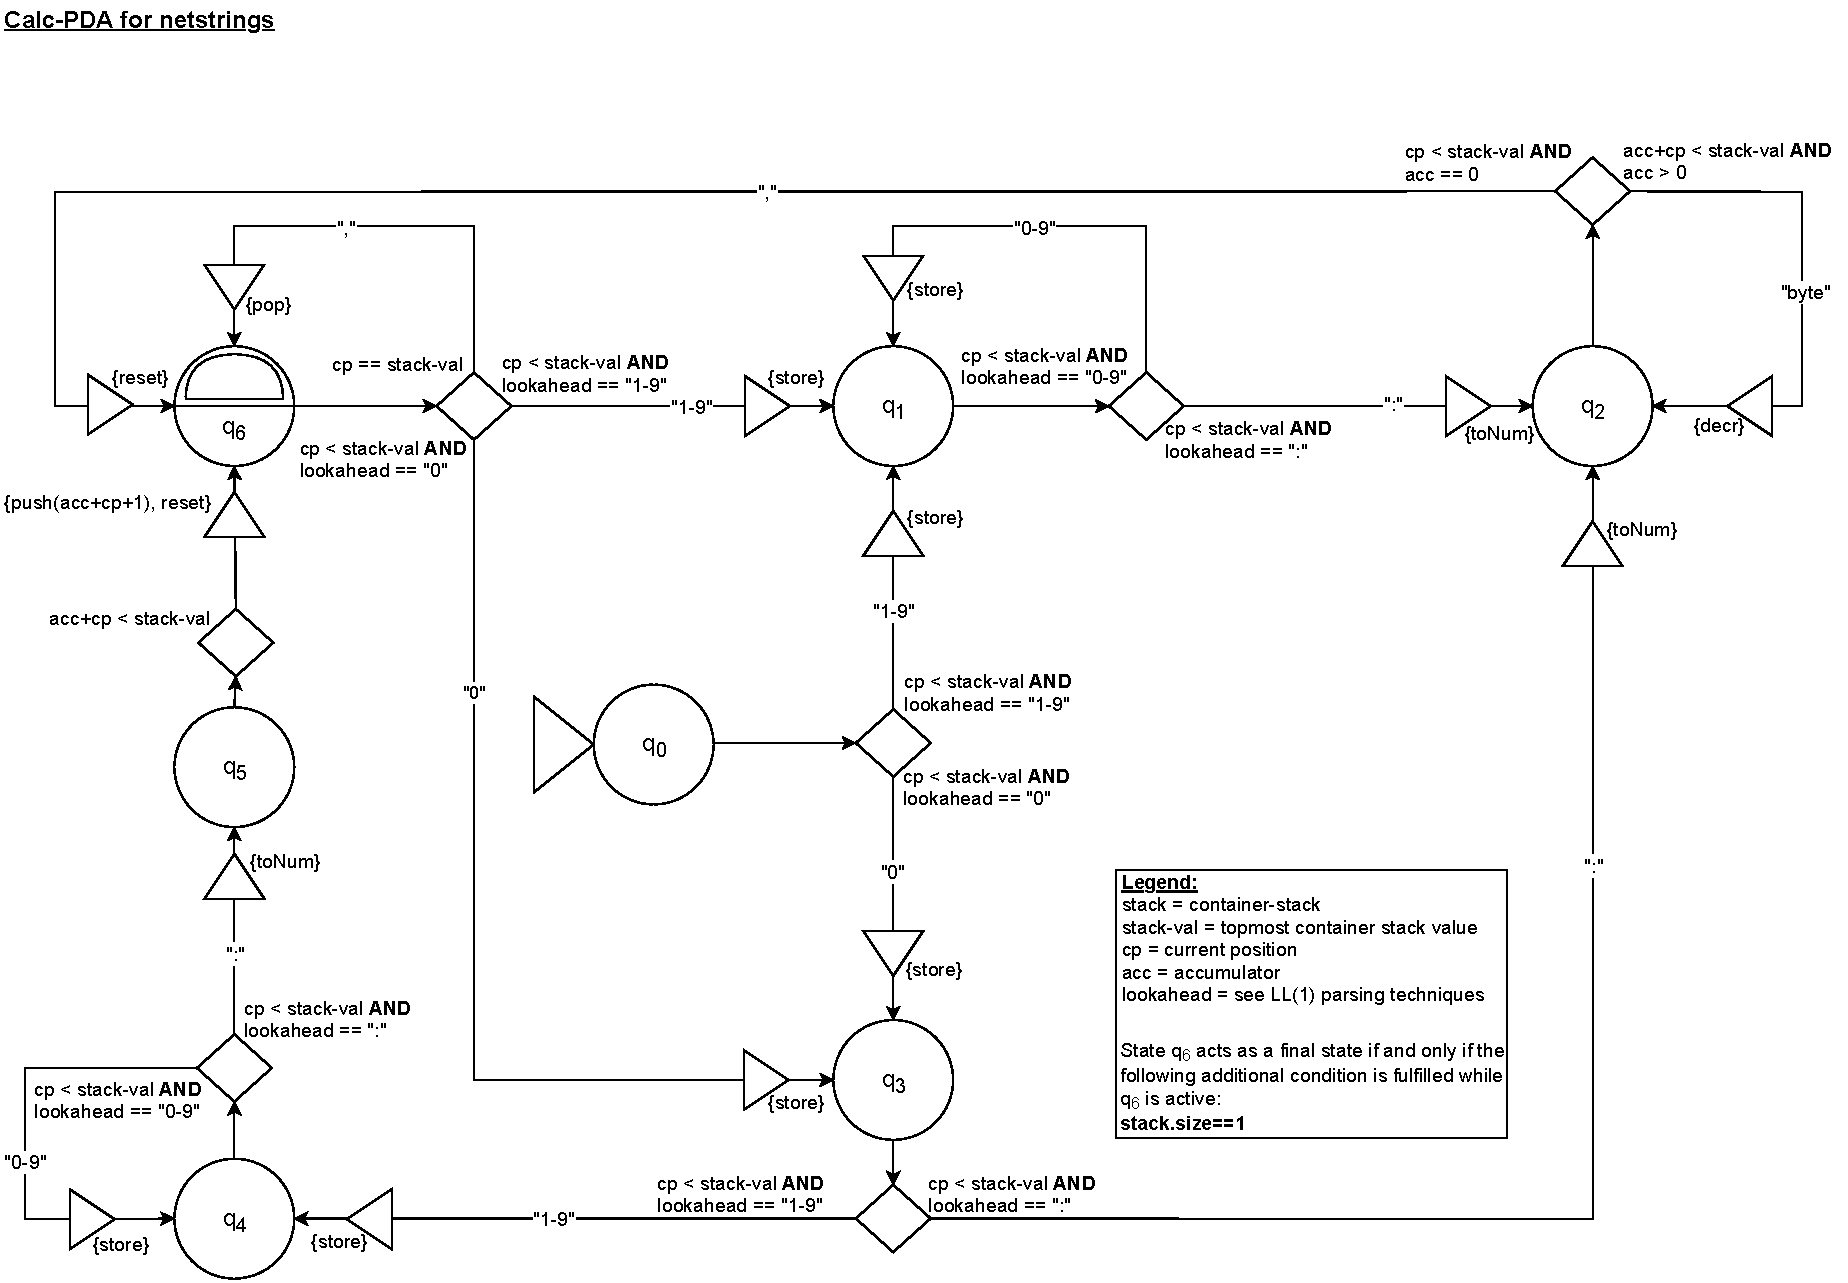
\includepdf[pages={1}]{fig/Calc-PDA-netstrings-version_10.pdf}
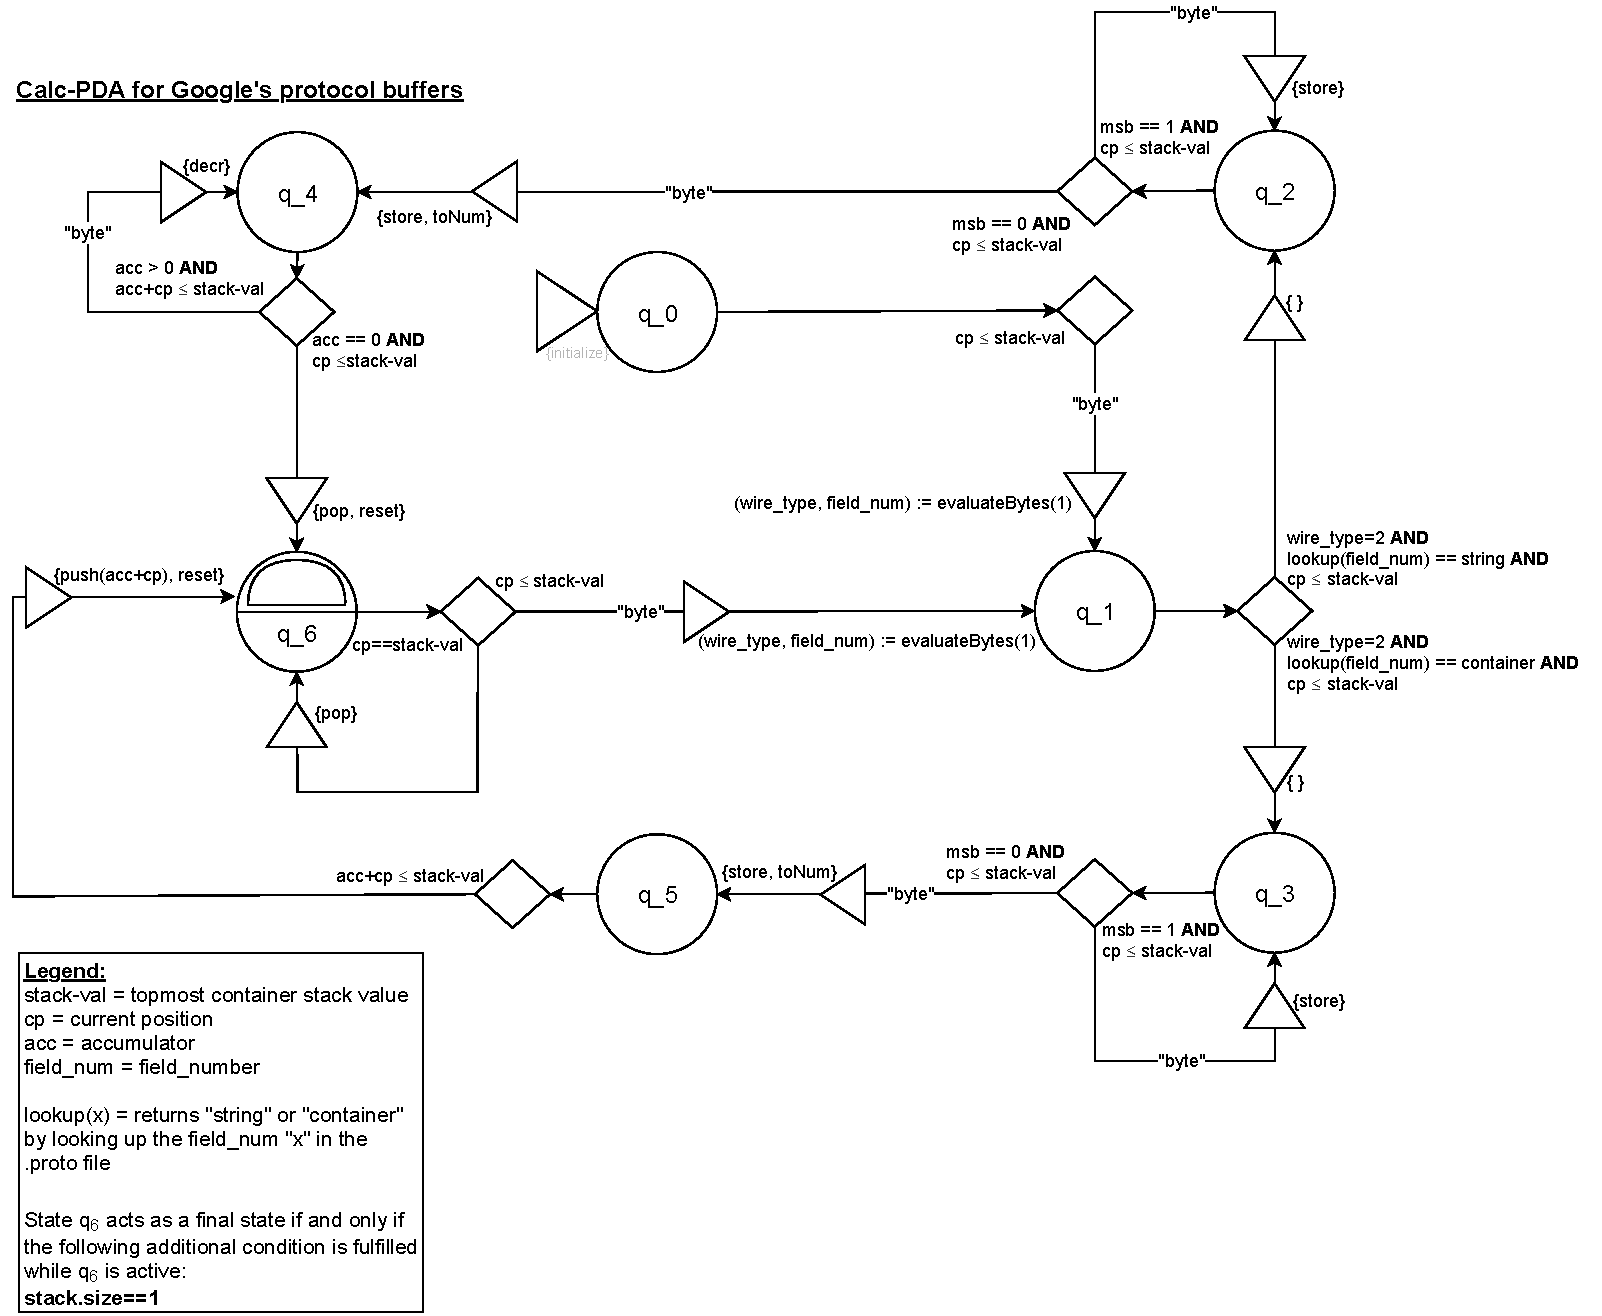
\includepdf[pages={1}]{fig/Calc-protobuf-PDA-version-7.pdf}

\end{document}
